\section{Introduction}
\label{sec-intro}

%Given a task and a social network $G(V, E)$, where $V$ is a set of experts labeled with skills and $E$ reflects the collaboration relations among the experts,
The {\em top-$k$ team formation} problem is to find a list of $k$ highly collaborative teams of experts such that every team satisfies the skill requirements of a certain task.
Various approaches~\cite{Lappas09,Kargar11,ArisLuca12,GajewarS12,realTeamForm13,SamikKVM12} have been proposed,
and fall into two categories in terms of the way to improve the collaborative compatibility of team members:
 (a) minimizing team communication costs,
defined with \eg the diameter, minimum spanning tree and the sum of pairwise member distances of the induced subgraph~\cite{Lappas09,Kargar11,ArisLuca12,SamikKVM12}, and
(b) maximizing team communication relations,
\eg the density of the induced subgraph~\cite{GajewarS12,realTeamForm13}.
Further, \cite{GajewarS12} and \cite{realTeamForm13} consider a practical setting by introducing a lower bound on the number of individuals with a specific skill in a team, and an upper bound of the total team members, respectively.




\begin{example}
\label{exm-motivation}
Consider a recommendation network $G_1$ taken from \cite{TerveenM05} as depicted in Fig.~\ref{fig-motivation-example},
in which (a) a node denotes a person labeled with her expertise, \eg project manager (\kw{PM}), software architect (\kw{SA}), software developer (\kw{SD}), software tester (\kw{ST}),
user interface designer (\kw{UD}) and business analyst (\kw{BA}),
and (b) an edge indicates the collaboration relationship between two persons, \eg ($\kw{PM_{1}}$, $\kw{UD_{1}}$) indicates $\kw{PM_{1}}$ worked well with $\kw{UD_{1}}$ within previous projects.

A headhunt helps to set up a team for a software product by searching proper candidates from $G_1$ (ignore dashed edges).
A desired team has
(i) one \kw{PM}, and one to two \kw{BAs}, \kw{UDs}, \kw{SAs}, \kw{SDs} and \kw{STs}, such that
(ii) \kw{PM} should collaborate with \kw{SAs}, \kw{BAs} and \kw{UDs} well, and \kw{SDs} and \kw{STs} should collaborate with each other well and both with \kw{SAs} well.

\eat{
One may want to look for candidate teams with existing methods,
 (1) by minimizing the {\em team diameter} \cite{Lappas09},
which returns the team with $\{\kw{BA_3}$, \kw{PM_3}, \kw{UD_4}, \kw{SA_4}, \kw{SD_4}, $\kw{ST_4}\}$,
(2) by minimizing the {\em sum of all-pair distances} of teams \cite{Kargar11},
which returns exactly the same team as (1) in this case,
or (3) by maximizing the {\em team density} \cite{GajewarS12}, which returns the team consisting of the nodes of the two connected components in $G_1$ with \kw{PM_1} and \kw{BA_3} (excluding \kw{UD_2}, \kw{PM_3}, \kw{UD_4}, \kw{SA_4}).

However, one may notice that these teams only satisfy the skill requirement, and cannot guarantee  the specific collaboration relationships among team members, \ie structural constraints. Indeed, the team found in (1) and (2) is connected by \kw{BA_3} only, and the team found in (3) has loose collaborations among its members.
Further, the capacity constraint in \cite{GajewarS12,realTeamForm13} needs to be extended to express the capacity bounds here.
That is, existing methods are not appropriate for identifying the above desired teams.
}%%%EAT

One may verify that existing methods \cite{Lappas09,Kargar11,GajewarS12,realTeamForm13}, can hardly find a desired team.
They only find teams satisfying the skill requirement~\cite{Lappas09,Kargar11,GajewarS12} and the lower bound capacity requirement~\cite{GajewarS12,realTeamForm13}  (condition (i)), and cannot guarantee  the specific collaboration relationships among team members, \ie structural constraints (condition (ii)).
 \end{example}

\eat{ It is because existing methods fall short of capturing the collaboration relations between specific team members, \ie the topology constraint (condition (2)).
However, in practice, it is rather important to take the functionality of different members into consideration~\cite{MerzSeeber15};
and few of them consider the capacity constraint (in condition (1)), and even consider, they always focus on the lower bounds~\cite{GajewarS12}, which results in a large quantity.

 and the number of team members is less than the cardinality requirement of the task
One can verify none of existing methods suffice to express the above requirements.

One can find none of the teams could work well in practice: the team found by (a) and (b) is connected by only one member \kw{BA} and the number of team members is less than the cardinality requirement of the task;
and the size of the team found by (c) is too large. It is because existing methods fall short of capturing the collaboration relations between specific team members, \ie the topology constraint (condition (2)).
However, in practice, it is rather important to take the functionality of different members into consideration~\cite{MerzSeeber15};
and few of them consider the capacity constraint (in condition (1)), and even consider, they always focus on the lower bounds~\cite{GajewarS12}, which results in a large quantity.}%%%EAT


\eat{
A natural question is how to further capture the {\em structural and capacity constraints} in a unified model for team formation?
We essentially introduce a revision of graph pattern matching, an extension of graph simulation~\cite{infsimu95} and strong simulation~\cite{MaCFHW14}, for team formation to fill in this gap.
}%%%EAT

A natural question is how to further capture the {\em structural and capacity constraints} in a unified model for team formation?
We  introduce a revision of {\em graph pattern matching} for team formation to fill in this gap.
%
Given a pattern graph $P$ and a data graph $G$, graph pattern matching is to find all subgraphs in $G$ that match $P$, and has been extensively studied~\cite{Ullmann76,infsimu95,FanLMTWW10,MaCFHW14,Guanfeng15,FanCount16}.  Essentially, we utilize patterns to capture the structural constraint, and revise the semantics of graph pattern matching for team formation. For instance, a desired team requirement can be specified by the pattern $P_1$ (ignore dashed edges) in Fig.~\ref{fig-motivation-example}, in which nodes represent the skill requirements,  edges specify the topology constraint, and the bounds on nodes are the capacity constraint.

%Especially, {\em strong simulation} introduces duality and locality into simulation, and shows a good balance between its computational complexity and its ability to preserve graph topology~\cite{MaCFHW14}.


Another issue lies in that team formation is accompanied with a highly dynamic environment. It typically needs many efforts to find the ideal teams, and is common for professionals to refine patterns  (requirements) multiple rounds~\cite{SajjadPG12,HabibiP15}. Further, real-life graphs are often big and constantly evolve over time~\cite{FanWW13-tods}. We show this with an example.


\begin{figure}[tb!]
\vspace{-2ex}
\begin{center}
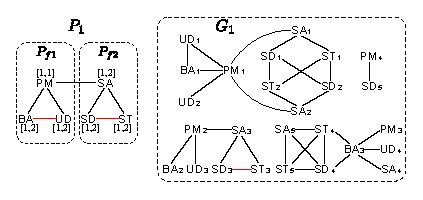
\includegraphics[scale=1.15]{./fig/motivation-example.eps}
\end{center}
\vspace{-3ex}
\caption{Motivation example}
\label{fig-motivation-example}
\vspace{-4ex}
\end{figure}



\begin{example}
\label{exm-motivation-inc}
Consider $P_{1}$ and $G_{1}$ in Example~\ref{exm-motivation} again.
	
\sstab{(1)} % When the manager gets the match result, \ie the top-$k$ teams $P_{1}(G_{1})$ to $P_{1}$ in $G_{1}$,
One may find that $P_1$ is too restrictive to find any sensible match in  $G_{1}$.
Hence, she needs to refine the pattern by updating $P_1$ with $\Delta P_{1}$, \eg an edge
deletion $(\kw{SD},\kw{ST})^-$.
%We denote $P_{1}\oplus\Delta P_{1}$ the updated pattern.
%It is much better to derive $P_{1}\oplus\Delta P_{1}(G_{1})$ from $P_{1}(G_{1})$
%than a computation for $P_{1}\oplus\Delta P_{1}$ in $G_{1}$ from scratch.
%\looseness=-1
	
\sstab{(2)} It is also common that a data update $\Delta G_1$ comes on $G_1$, \eg an edge insertion $(\kw{SD_3},\kw{ST_3})^+$.
%Similar with (1), it is better to compute $P_{1}(G_{1}\oplus\Delta G_{1})$ from $P_{1}(G_{1})$ incrementally.
	
\sstab{(3)} Finally, it can be the case when pattern update $\Delta P_{1}$  and data update $\Delta G_{1}$ come simultaneously on $P_1$ and $G_1$.
%,  $P_{1}\oplus\Delta P_{1}(G_{1}\oplus\Delta G_{1})$ from $P_{1}(G_{1})$ incrementally
\end{example}

This motivates us to study the {\em dynamic top-k team formation} problem, to handle continuous
pattern and data updates, separately and simultaneously. It is known that incremental algorithms avoid re-computing from scratch by re-using previous results~\cite{inc-survey}. However, incremental algorithms of graph pattern matching for pattern updates has not been investigated, though there exist incremental algorithms of graph pattern matching for dealing with data updates~\cite{FanLMTWW10,FanWW13-tods,FanHT17}.
Further, it is also challenging for incremental algorithms to handle simultaneous pattern and data updates  in a unified way.



\eat{
often too costly to recompute top-$k$ teams from scratch in response to pattern and data updates.
These highlight the need for incremental algorithms to compute the updated top-$k$ teams.
As opposed to batch algorithms, incremental algorithms avoid re-computing from scratch by re-using previous results.
Traditional incremental algorithms for graph queries including graph pattern matching queries are proposed to compute changes in response to data updates, which has a lot of work~\cite{FanLMTWW10,FanWW13-tods,FanHT17}.
However, the study on incremental algorithms for graph pattern updates is in its vacancy.

Given a pattern graph $P$ and a data graph $G$, the graph pattern matching results $P(G)$ in $G$ for $P$ and changes $\Delta G$ to $G$ as input,
the traditional incremental matching problem is to compute changes $\Delta O$ to $P(G)$ such that $P(G\oplus\Delta G)$=$P(G)\oplus \Delta O$.
Here $\oplus$ denotes applying changes $\Delta S$ to $S$, when $S$ is data graph $G$ or query result $P(G)$.
It is to improve response time by reducing computations on big $G$ to small $\Delta G$ and $\Delta O$.

As a basis of \dynteamF, we also investigate the incremental problem for graph pattern matching on pattern updates.
The definition can be formulated along the same line with existing data incremental problems.
%different with data incremental algorithms that preserve some desirable properties that the recomputation can be {\em bounded}  by the changes in the input and output as the impact of data updates can be localized~\cite{Reps96, FanLMTWW10,FanWW13-tods,FanHT17},
However, devising pattern incremental algorithms is quite challenging as the impact of pattern updates is global,
due to the inherent hardness of the problem.
Despite of this, we devise an effective unified incremental approach for the \dynteamF\, problem.

 }%%%EAT






\looseness = -1

\stitle{Contributions}. To this end,  we introduce a graph pattern matching approach for (dynamic) top-$k$ team formation.


\stab (1) We propose {\em team simulation}, a revision of traditional graph pattern matching, for top-$k$ team formation (Section~\ref{sec-tsim}).
It extends existing methods by incorporating the structural and capacity constraints using pattern graphs.
To cope with the highly dynamic environment of team formation, we also formulate the dynamic top-$k$ team formation problem  (Section~\ref{sec-tsim}), for dealing with pattern and data updates, separately and simultaneously.




\stab (2) We develop a batch algorithm for computing top-$k$ teams via team simulation (Section~\ref{sec-tsimAlg}).
We study the satisfiability problem for pattern graphs, a new problem raised in the presence of capacity bounds for graph pattern matching.
We also propose two optimization techniques, handling radius varied balls and density based filtering, for speeding up the process of computations.



\stab (3) We develop a unified approach to handling the need for both pattern and data updates (Sections~\ref{sec-dynamictopk} and~\ref{sec-IncAlg}).
Due to the inherent difficulty of the problem, we propose an incremental strategy based on {\em pattern fragmentation} and {\em affected balls} by localizing the effects of pattern and data updates, and we develop a unified incremental algorithm for dealing with separate and simultaneous pattern and data updates,
with an optimization technique with the {\em early return} property for incremental top-$k$ algorithms, an analogy of the traditional early termination property.


\eat{%%%%%%%%%%%%%%%%move to section 3

As opposed to batch algorithms that recompute new match results from scratch,
incremental algorithms \cite{inc-survey} have been proposed to compute new match results,
by reusing and updating previous cached results according to the changes in input.
\looseness=-1

\begin{example}
\label{exm-motivation-inc}
Recall $P_{1}$ and $G_{1}$ in Fig.~\ref{fig-motivation-example} and continue.

\sstab{(1)} When the user gets the matched teams $P_{1}(G_{1})$ to $P_{1}$ in $G_{1}$, she may find $P_1$ is too restrictive to find possible teams.
Therefore, she enters pattern updates $\Delta P_1$ on $P_1$, composed of an edge deletion $(\kw{SD},\kw{ST})^-$.
We denote $P_{1}\oplus\Delta P_{1}$ the revised pattern.
It is much better to derive $P_{1}\oplus\Delta P_{1}(G_{1})$ from $P_{1}(G_{1})$
than a computation for $P_{1}\oplus\Delta P_{1}$ in $G_{1}$ from scratch.
\looseness=-1

\sstab{(2)} When data updates $\Delta G_1$ come on $G_1$, composed of an edge insertion $(\kw{SD_3},\kw{ST_3})^+$.
Similarly with (1), it is better to compute $P_{1}(G_{1}\oplus\Delta G_{1})$ from $P_{1}(G_{1})$ incrementally.

\sstab{(3)} Even better, when it comes to the case pattern $\Delta P_{1}$ and data updates $\Delta G_{1}$ come together, it is desirable to compute $P_{1}\oplus\Delta P_{1}(G_{1}\oplus\Delta G_{1})$ from $P_{1}(G_{1})$ incrementally.
\end{example}
}%%%%%%%%EAT



\eat{%%%EAT
%Hence, there is an urgent need to study the team formation problem in a dynamic setting.
These encourage us to propose the {\em dynamic top-$k$ team formation} problem (\dynteamF),
to handle separate and simultaneous pattern and data updates.
However, the problem is non-trivial.
There has been a bunch of work on data incremental algorithms on graphs~\cite{Reps96,FanWW13-tods},
but less work on handling pattern updates is known, and furthermore less work on handling both data and pattern updates is known. The challenges comes from three aspects:
(a) the nature of pattern updates, pattern updates have significant impacts on the match results.
A unit update is likely to result in the entire change in match results, such that all previous match results need to be re-computed, which is actually a costly batch computation;
(b) the demand to design light weight and effective auxiliary data structures for the dynamic team formation problem, concerning the space consumption and the efficiency;
and (c) the requirement to design a {\em one-method-fits-two} model, to support pattern and data updates simultaneously and separately.

To solve the {\em top-$k$ team formation} problem and the {\em dynamic top-$k$ team formation} problem, several fundamental problems call for a full treatment.
(1) How to extend graph pattern matching for top-$k$ team formation to retain the properties in existing methods, and pursue more practical usage,
%such as combine capacity bound and structural constraints on matched results,
without sacrificing the efficiency?
(2) How to efficiently support pattern updates for, \eg user query adjustments on patterns, by reusing previous cached results as much as possible?
(3) How to handle data updates to meet the practical requirements?
(4) How to design a unified incremental model to handle both pattern and data updates efficiently in a simultaneous manner?
}%%%EAT

\eat{
\stitle{Contributions}. To this end,  we introduce a graph pattern matching approach for (dynamic) team formation.

\stab (1) We propose {\em team simulation} for top-$k$ team formation, a revision of traditional graph pattern matching,
which extends existing methods {\em strong simulation} for team formation by incorporating the structural and capacity constraints using pattern graphs  (Section~\ref{sec-tsim}).
We also study the satisfiability problem for pattern graphs, a new problem raised in the presence of capacity bounds for graph pattern matching.
We finally develop an efficient cubic batch algorithm with two optimization techniques, \ie density based filtering and pattern minimization, for computing top-$k$ teams via team simulation.

\stab (2) We formulate the dynamic top-$k$ team formation problem, and develop a unified approach to handling the need for both pattern and data updates (Sections~\ref{sec-dynamictopk} \& \ref{sec-IncAlg}).
We first prove that the  problem is unbounded even for single pattern or data updates, by extending the notion of incremental boundedness~\cite{Reps96}.
In light of this, we then propose an incremental strategy based on {\em pattern fragmentation} and {\em affected balls} to localize the effects of pattern and data updates. We finally develop a unified incremental algorithm for dealing with continuous pattern and data updates, separately and simultaneously,
with an optimization technique with the {\em early return} property for incremental top-$k$ algorithms, an analogy of the traditional early termination property.
}%%%EAT

\eat{%%%EAT
\stab (3) Using real-life and synthetic graphs, we experimentally verify the effectiveness and efficiency of the static and dynamic top-$k$ graph pattern matching model and optimization techniques, for separate and simultaneous pattern and data updates, for solving \teamF\,and \dynteamF\,problems.
{\bf Add details}
}%%%EAT

\stab (4) Using real-life data (\citationd) and synthetic data (\synthetic), we demonstrate the effectiveness and efficiency of our graph pattern matching approach for (dynamic) team formation (Section~\ref{sec-expt}).
We find that (a) our method is able to identify more sensible teams than existing team formation methods \wrt \eat{three} practical measurements,
and (b) our incremental algorithm outperforms our batch algorithm, even when changes reach 36\% for pattern updates, 34\% for data updates and (25\%, 22\%) for simultaneous pattern and data updates, and when 29\% for continuous pattern updates, 26\% for continuous data updates and (20\%, 18\%) for continuous simultaneous pattern and data updates, respectively.


To our knowledge, this work is among the first to study simultaneous pattern and data incremental computations, no previous work has studied pattern updates for incremental pattern matching~\cite{FanHT17,FanWW13-tods}, not to mention continuous and simultaneous pattern and data updates.  This is  the most general dynamic setting for incremental computations.

All detailed proofs are available  in the full version~\cite{fullvldb18}.

\stitle{Related work}. Previous work can be classified as follows.

%\etitle{Graph pattern matching}.

 Graph simulation \cite{infsimu95} and its extensions have been introduced for graph pattern matching~\cite{FanLMTWW10,MaCFHW14,Guanfeng15,FanCount16}, in which {\em strong simulation} introduces duality and locality into simulation~\cite{MaCFHW14}, and shows a good balance between its computational complexity and its ability to preserve graph topology. Furthermore, \cite{FanCount16} already adopts capacity bounds on the edges of pattern graphs via subgraph isomorphism, and \cite{FanWWXin13} uses graph pattern matching to find single experts, instead of a team of experts. In this study, team simulation is proposed for team formation as an extension of graph simulation and strong simulation on undirected graphs with capacity constraints on the nodes of pattern graphs.


%\etitle{Team formation}.

There has been a host of work on team formation by minimizing the communication cost of team members, based on the diameter, density, minimum spanning tree, Steiner tree, and sum of pairwise member distances among others \cite{Lappas09,Kargar11,ArisLuca12,GajewarS12,realTeamForm13,SamikKVM12,LiTongCao15}, which are essentially  a specialized class of keyword search on graphs~\cite{Aggarwal10}. Similar to~\cite{Kargar11}, we are to find top-$k$ teams. However, \cite{Kargar11} adopted Lawler's procedure \cite{Lawler1972}, and is inappropriate for large graphs. We also adopt {\em density}  as the communication cost, which shows a better performance~\cite{GajewarS12}, and further require that all team members are {\em close to each other} (located in the same balls), along the same line with~\cite{Lappas09,Kargar11,ArisLuca12,SamikKVM12}.
Except for simply minimizing the communication cost among team members,
\cite{HuangLv16,Kargar11} consider minimizing the cost among team members and team leaders.
Different from these work, we introduce {\em structural constraints}, in terms of graph pattern matching~\cite{FanLMTWW10,MaCFHW14}, into team formation, while retaining the capacity bounds on specific team members like~\cite{realTeamForm13,GajewarS12}.



%\etitle{Incremental computations}.

Incremental algorithms (see \cite{inc-survey,FanHT17} for a survey) have proven usefulness in a variety of applications,
and have been studied for graph pattern matching~\cite{FanLMTWW10,FanWW13-tods} and team formation \cite{ArisLuca12} as well.
However, \cite{inc-survey,FanHT17,FanLMTWW10,FanWW13-tods} only consider data updates,
and \cite{ArisLuca12} only considers continuous coming new tasks. In this work, we  deal with both pattern and data updates for team formation, and support both insertions and deletions. To our knowledge, this is the first study on pattern updates, and is the most general and practical dynamic setting considered so far.

{Query reformulation (\aka query rewriting) is to generate alternative queries that may produce better answers,
and has been studied for structured queries~\cite{MottinEmpty13}, keyword queries~\cite{YaoQReform12} and graph queries~\cite{MottinGReform15}.
However, different from our study of handling pattern updates, the focus of query reformulation is not on incremental computations.

%\etitle{Top-k queries}.

Although top-$k$ queries (see~\cite{IlyasBS08} for a survey) have been studied for both graph pattern matching and team formation~\cite{Kargar11},
they have never been studied for both team formation and graph pattern matching  in a dynamic setting.


\eat{
\etitle{Query reformulation}. \textcolor{blue}{Query reformulation (\aka query rewriting/modification) is to provide users with a set of specializations of the original query that may better capture their search intent.
It has been studied for structured queries~\cite{MottinEmpty13}, keyword queries~\cite{YaoQReform12} and graph queries~\cite{MottinGReform15}.
However, they all aim at automatically providing alternative queries (\eg supergraphs~\cite{MottinGReform15}) to users,
while care less about answering the changed queries.
In this work, we focus on handling query modification from users and how to quickly return the answers based on previous answers.}
}

\eat{%%%EAT
To retain the properties in existing methods, and pursue more practical usage, we incorporate the capacity bounds, density measure and locality into graph simulation as the matching semantics.

When a user inputs a pattern graph into a system with a data graph already stored in it, and gets the match result, sometimes he or she may find that the query is not appropriate in some sense after an analysis on the result. Then the user probably makes some small adjustments on the pattern graph. However, it is expensive to recompute the matches from scratch via batch algorithm due to the slight change in pattern graph, and this comes the convenience for executing incremental graph matching, which just computes changes in the match result corresponding to the updates in pattern graph.
}%%%EAT
